\chapter{Desenvolvimento}

\section{O SISTEMA PRINCIPAL}

O sistema principal, como explicado anteriormente, é o responsável pelo controle do braço que movimentará o transdutor do aparelho de ultrassom. O controle será feito pelo médico, que terá em mãos a carcaça, como visto da figura \ref{des_fig1}, com arduino e módulo sensor inercial dentro. O desenho técnico com as medições da carcaça estão presentes na figura \ref{des_fig1} a seguir.

\begin{figure}[H]
	\centering	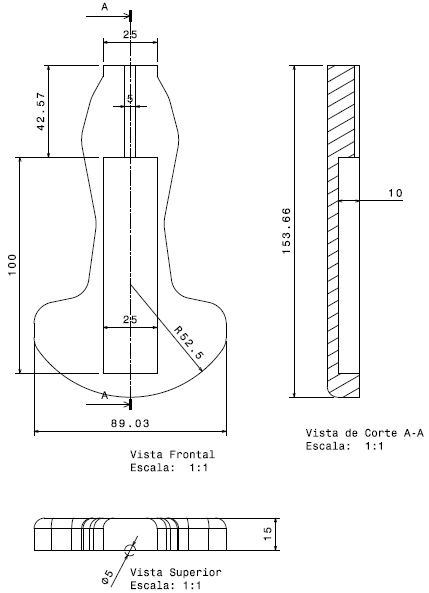
\includegraphics[keepaspectratio=true,scale=1]{figuras/medicas_controle.png}
	\caption{Dimensões da carcaça do módulo de controle}
	\label{des_fig1}
\end{figure}

Para fora da carcaça sairá apenas um cabo USB para a comunicação do Arduino com o computador da estação de controle. Os dados enviados do Arduino para o computador serão do tipo serial, assim, o programa no computador deve ler os dados seriais vindos da porta USB a qual o Arduino está conectado.

A escolha do sensor inercial ocorreu devido a proposta do produto ser o mais simples possível para a utilização do médico. Pressupondo que o médico especialista que realizará o exame possui experiência com aparelhos de ultrassom, o sistema de controle escolhido, facilita a utilização do produto, pois é semelhante a um transdutor real, sendo necessário apenas um breve tutorial de como o sistema funciona para a utilização do aparelho.

Esse sensor inercial envia ao Arduino 7 sinais:
\begin{itemize}
\item 3 eixos de acelerômetro (movimento de translação nos eixos x,y e z);
\item 3 eixos de giroscópio (movimento de rotação nos eixos x, y e z);
\item 1 sinal de temperatura do ambiente.
\end{itemize}

Sendo assim, é possível enviar estes pacotes de dados para os motores na estação de exame onde o paciente se encontra, fazendo com que a combinação dos 6 sinais de movimentação controle os motores do braço mecânico, sendo necessário realizar um processamento de sinais para enviar as informações corretas para cada motor existente nos eixos do braço mecânico.
    Para o módulo sensor inercial, têm-se como principal critérios de escolha o módulo ter giroscópio, acelerômetro e ser compatível com a plataforma Arduino \cite{bergmuller2015desenvolvimento}. Com base nesse critério, foram selecionados os seguintes componentes:

\begin{itemize}
\item \textbf{MPU-6050}
	\begin{itemize}
		\item Tensão de Operação: 2,375 – 3,46V
		\item Faixa de Giroscópio: +/- 250, 500, 1000 e 2000 graus/segundo
		\item Faixa de Aceleração: +/- 2g, +/- 4g, +/- 8g, +/- 16g
		\item Dimensões: 16 mm x 21 mm
		\item Preço Médio:  R\$ 20,00
	\end{itemize}
\begin{figure}[H]
	\centering	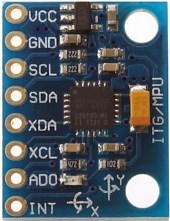
\includegraphics[keepaspectratio=true,scale=1]{figuras/MPU-6050.jpg}
	\caption{Módulo MPU-6050 (sensor inercial)
}
	\label{des_fig2}
\end{figure}
\end{itemize}    



\begin{itemize}
\item \textbf{GY-80}
\begin{itemize}
\item Tensão de Operação: Mínima=3V , Máxima=5V
\item Faixa de Giroscópio: +/- 250, 500 e 2000 graus/segundo
\item Faixa de Aceleração: +/- 2g, +/- 4g, +/- 8g, +/- 16g
\item Dimensões: 25.8 mm x 16.8 mm
\item Preço Médio:  R\$ 100,00
\end{itemize}
\begin{figure}[H]
	\centering	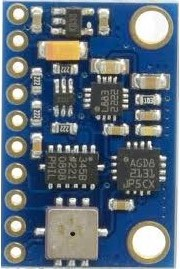
\includegraphics[keepaspectratio=true,scale=1]{figuras/GY-80.jpg}
	\caption{Módulo GY-80 (sensor inercial)}
	\label{des_fig3}
\end{figure}
\end{itemize}

Ao analisar as opções disponíveis e a suas especificações técnicas dos sensores acelerômetro e giroscópio, foi visto que ambos os módulos operam com critérios idênticos, ou muito próximos, entretanto, ao considerar dimensão, preço e tensão de operação, a melhor escolha é o MPU-6050, sendo assim, o escolhido como o módulo de sensor inercial.

Para a escolha do Arduino, os critérios avaliados foram: possuir uma entrada USB/mUSB para saída dos dados seriais, ter dimensões mínimas e possuir pinos para conexão do módulo sensor inercial escolhido, conforme a \ref{des_fig4}. Com base nestes critérios, optou-se pelo Arduino Nano como melhor escolha, visto que outros modelos ou tem USB integrado, mas são grandes, ou tem dimensões mínimas, mas não possui conexão USB para a comunicação serial com o computador. Sendos as especificações do Arduino Nano \cite{arduinonano}:

\begin{itemize}[noitemsep]
\item Microcontrolador: ATmega328
\item Tensão de operação (nível lógico): 5V
\item Tensão de entrada (recomendada): 7-12V
\item Tensão de entrada (limites): 6-20V
\item Pinos digitais I/O: 14, dos quais 6 podem ser saídas PWM
\item Pinos de entrada analógica: 8
\item Corrente contínua no pino I/O: 40 mA
\item Memória Flash: 16KB (dos quais 2KB são utilizados pelo bootloader)
\item SRAM: 1KB
\item EEPROM: 512 bytes
\item Velocidade de clock : 16 MHz
\item Dimensões:  18.5mm x 43.2mm
\begin{figure}[H]
	\centering	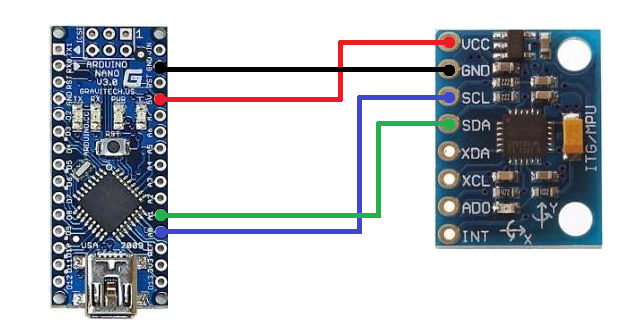
\includegraphics[keepaspectratio=true,scale=0.8]{figuras/conex_nano_mpu.png}
	\caption{Conexão entre Arduino Nano e Módulo MPU-6050}
	\label{des_fig4}
\end{figure}
\end{itemize}

Para alimentar energeticamente os sistema principal, como foi descrito anteriormente, vai ser utilizada energia por meio de tomadas de 110V ou 220V, entretanto, funciona sob uma faixa de tensão de entrada de 6-20V com corrente contínua, entretanto trabalha em uma faixa recomendada de 7-12V; uma tensão abaixo de 7V pode ficar instável,já se for alimentado com tensões acima de 12V o regulador de tensão dentro do arduino pode superaquecer e danificar a placa. Portanto, como o projeto será realizado com o uso das tomadas de corrente alternada, há a necessidade, como já dito, de proteger o arduino, para isso será utilizado um transformador que leve a tensão de 110V ou 220V para a faixa de tensão do arduino a fim de corrigir a alta tensão recebida da tomada e será utilizado também um circuito retificador de onda para deixar a corrente em forma de corrente contínua \cite{sadikualexander2013}.

Entretanto, por segurança do médico e do paciente, caso ocorra algum erro na fonte energética principal, foi pensada uma segunda fonte energética para suprir o consumo energético do módulo principal, sendo essa fonte uma bateria. A bateria escolhida foi a Moura Nobreak VRLA 12MVA-7, pois a potência nominal suporta o arduíno em funcionamento, possui um preço razoável para a execução do projeto, é segura e confiável, possui alto desempenho e eficiência e é indicada para equipamento médico-hospitalares.

Essa bateria é uma composta de chumbo ácido regulada por válvulas com 12V de tensão e capacidade nominal de 7ah/hora, possui dimensões de 9,4cm x 6,5cm x 15,10 cm (altura x largura x comprimento) e um circuito interno nobreak. O média de preço de 64,49 reais \cite{mlbateriamoura}.

\begin{figure}[H]
	\centering	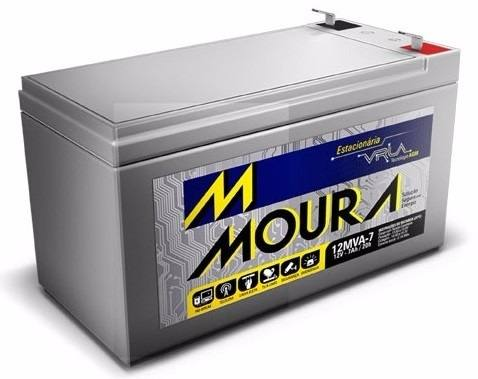
\includegraphics[keepaspectratio=true,scale=0.4]{figuras/bateria_moura.jpg}
	\caption{Bateria Moura chumbo ácido 12V}
	\label{des_fig5}
\end{figure}

\section{O SISTEMA ESCRAVO}

O braço mecânico desenvolvido, semelhante ao esquema representado pela figura 1, constitui-se por uma base fixa posicionada ao centro, sobre a qual é fixada uma haste a partir de uma junta do tipo rotativa torcional, que permite a rotação da mesma em torno do seu próprio eixo. A segunda junta possui a configuração rotativa rotacional e é posicionada entre a haste fixa e o braço, permitindo que haja a rotação do braço de forma perpendicular ao eixo de rotação da junta. A terceira junta promove a ligação entre o braço e o punho (antebraço) e é também do tipo rotativa rotacional, pois permite a rotação do punho em relação ao eixo perpendicular de rotação da junta. Na ponta do punho está o pulso, no qual será posicionado o transdutor sob a ação de masi uma junta rotativa rotacional e outra revolvente, esta última permite a rotação do transdutor em torno do eixo do pulso.

    Em notação de robótica, o braço mecânico possui a configuração TRR:RV, em que “T” representa a junta rotacional torcional, “R” a junta rotativa rotacional e “V” a junta revolvente; o sinal “:” indica que em seguida está representada a junta que acompanha o pulso.
    
    O arranjo estrutural adotado constitui a configuração mais próxima possível do que seria um braço humano (braço, antebraço e pulso), além de ser o mais versátil dentre os braços robóticos pela maior possibilidade de movimentos em um espaço reduzido. Esse braço, modela a partir do software Catia V5R19, o braço mecânico e seus respectivos movimentos (em amarelo 1,2 e 3) de rotação, aonde 1 corresponde a junta rotativa torcional, 2 a rotacional do braço e 3 a rotacional do punho e pode ser visto na figura \ref{des_fig6} a seguir.

\begin{figure}[H]
	\centering	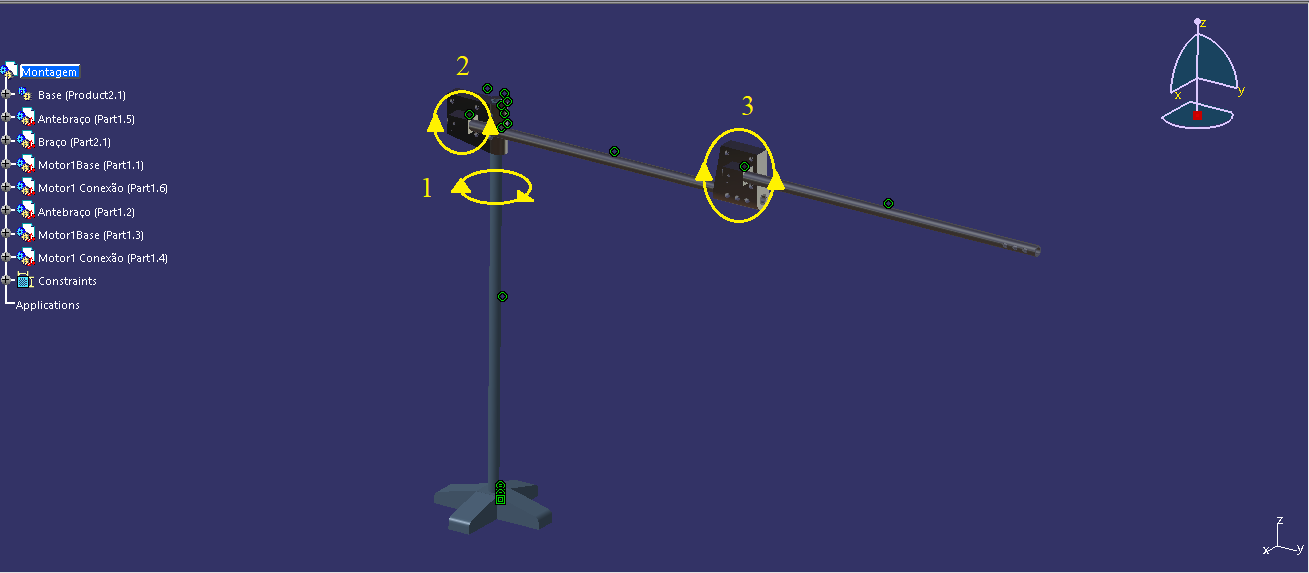
\includegraphics[keepaspectratio=true,scale=0.4]{figuras/braco_mecanico_2.png}
	\caption{Braço mecânico modelado a partir do software Catia V5R19.}
	\label{des_fig6}
\end{figure}
 As dimensões adotadas para o comprimento das hastes foram de 700 mm para a haste fixa à base, 300 mm para a haste que compõe o braço e 300 mm para a haste do antebraço. O diâmetro externo escolhido para a haste fixada à base foi de 19 mm e o diâmetro interno de 13 mm. Para o braço e o antebraço, as medidas dos diâmetros externo e interno permanecem iguais a da haste da base, para facilitar o encaixe nas juntas descritas anteriormente. Estas, na modelagem, foram construídas de tal forma que comportassem motores de passo Nema 23, responsáveis por exercer o movimento de rotação das hastes em cada junta. Uma imagem do encaixe modelado no mesmo software (Catia V5R19) pode ser visualizada na Figura \ref{des_fig7} a seguir.

\begin{figure}[H]
	\centering	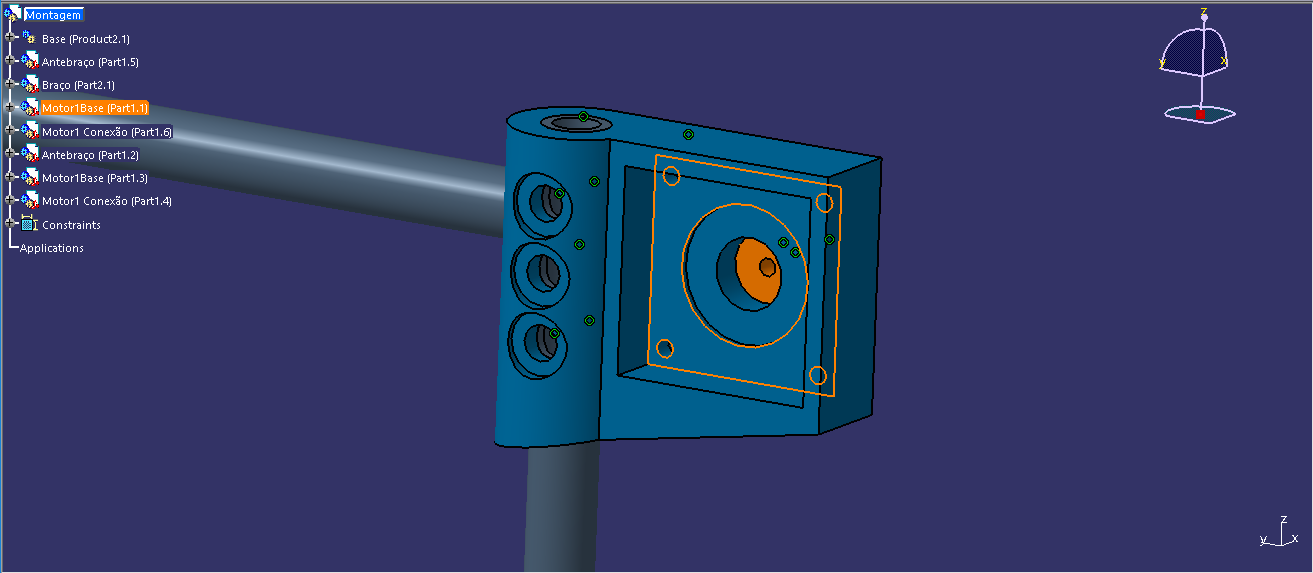
\includegraphics[keepaspectratio=true,scale=0.4]{figuras/braco_mecanico_3.png}
	\caption{Junta rotativa rotacional entre a haste fixa conectada à base e o braço. Na figura, está em evidência o encaixe modelado para um motor de passo Nema 23, responsável pelos movimentos de rotação. Em laranja, ao meio, está a conexão do motor com as hastes.}
	\label{des_fig7}
\end{figure}
Todas as dimensões foram determinadas de maneira prévia, com base na necessidade do braço em movimentar o transdutor de forma eficiente sobre uma área semelhante à compreendida pelo torso humano. A área foi calculada com base nos dados antropométricos da Tabela HDA (Henry Dreyfuss Associates, 2002) para a população norte-americana, por meio da qual considerou-se o percentil 97,5\% da população masculina adulta \cite{alvintilley2007}. Para calcular uma área de alcance para o braço mecânico, foram tomadas as medidas da altura dos ombros em relação ao quadril (homem em pé), igual a 18,1” (aproximadamente 46 cm), e a largura entre os ombros (em pé), equivalente a 15,2” (aprox. 39 cm), constituindo um “retângulo de alcance” para o braço de proporções 46x39 cm.

As juntas associadas à cada haste, como fora descrito, comportam motores de passo Nema 23 e tornam possíveis os movimentos de rotação. Neste caso, consistem essencialmente na base para o motor e em suas conexões com as hastes. As medidas para cada uma delas são descritas pelas Figuras \ref{des_fig8} e \ref{des_fig9} a seguir.

\begin{figure}[H]
	\centering	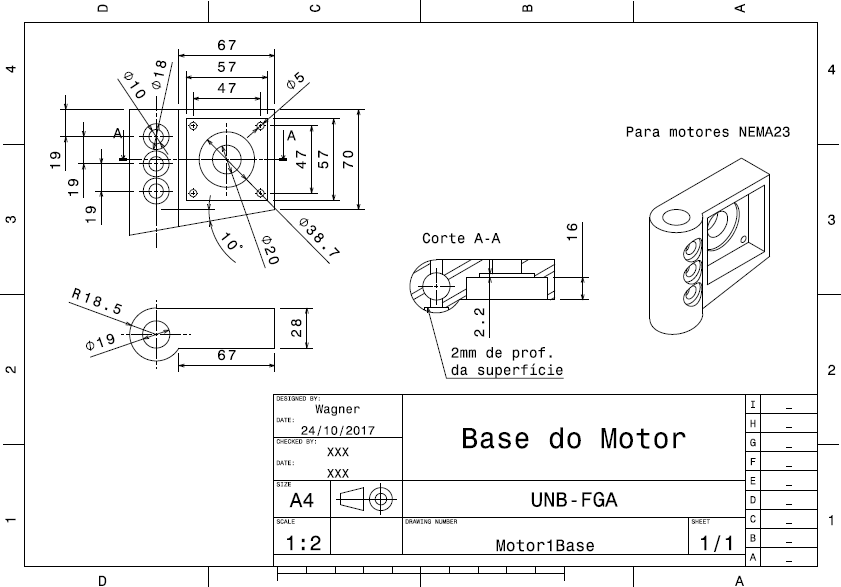
\includegraphics[keepaspectratio=true,scale=0.6]{figuras/braco_mecanico_4.png}
	\caption{Desenho técnico contendo as medidas da base do motor, uma das partes constituintes da junta}
	\label{des_fig8}
\end{figure}
\begin{figure}[H]
	\centering	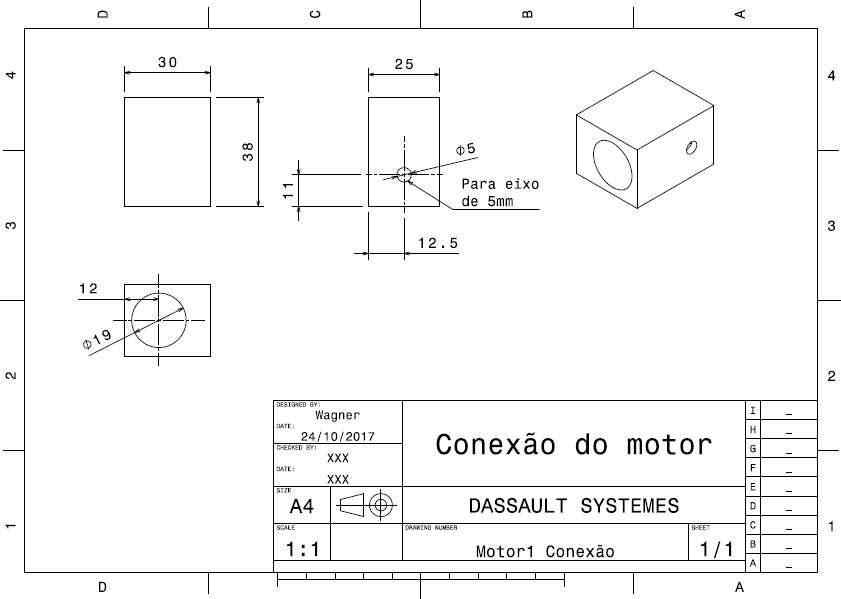
\includegraphics[keepaspectratio=true,scale=0.6]{figuras/braco_mecanico_5.png}
	\caption{Desenho técnico contendo as medidas da conexão do motor com as hastes, onde serão produzidos os movimentos de rotação na junta}
	\label{des_fig9}
\end{figure}
A base da estrutura, no caso, é composta por duas peças posicionadas de forma perpendicular uma sobre a outra, fixas por meio de um ajuste forçado. A estrutura contém um furo ao centro que permite a fixação da haste vertical, também acoplada pelo uso de um ajuste forçado. Este formato para a base foi escolhido pela facilidade de fabricação, simplicidade e grande inércia de rotação em todas as direções, além de possuir pouca massa e possibilitar o uso do mesmo material em que são construídas as juntas \cite{bracomec}. As medidas referentes às duas peças que formam a base estão indicadas na Figura \ref{des_fig10} a seguir.

\begin{figure}[H]
	\centering	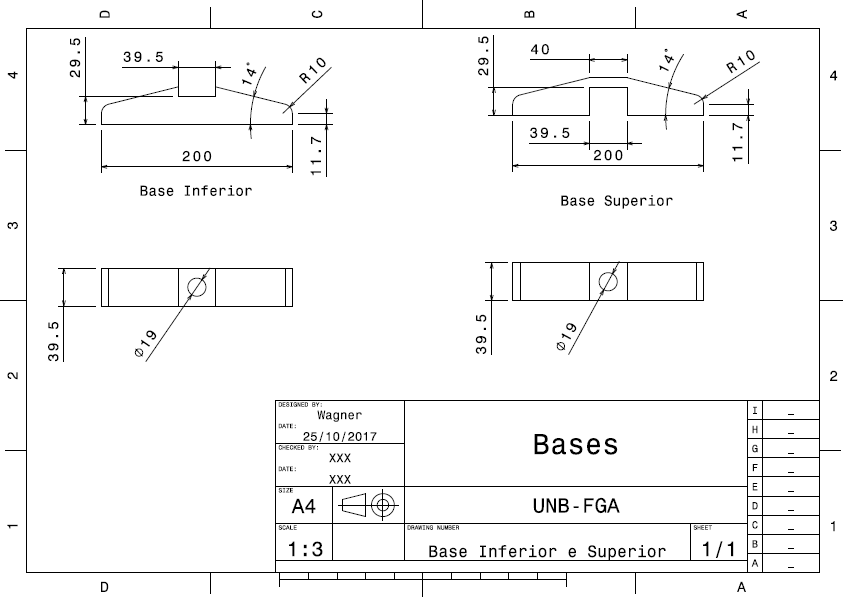
\includegraphics[keepaspectratio=true,scale=0.65]{figuras/braco_mecanico_6.png}
	\caption{Desenho técnico contendo as medidas das peças que constituem a base do braço.}
	\label{des_fig10}
\end{figure}
A montagem final do braço mecânico consiste     na integração entre a base fixa, as 3 hastes rígidas e a as juntas rotativas (com a base e a conexão dos motores). A Figura \ref{des_fig11} a seguir mostra a disposição das peças em um plano bidimensional:

\begin{figure}[H]
	\centering	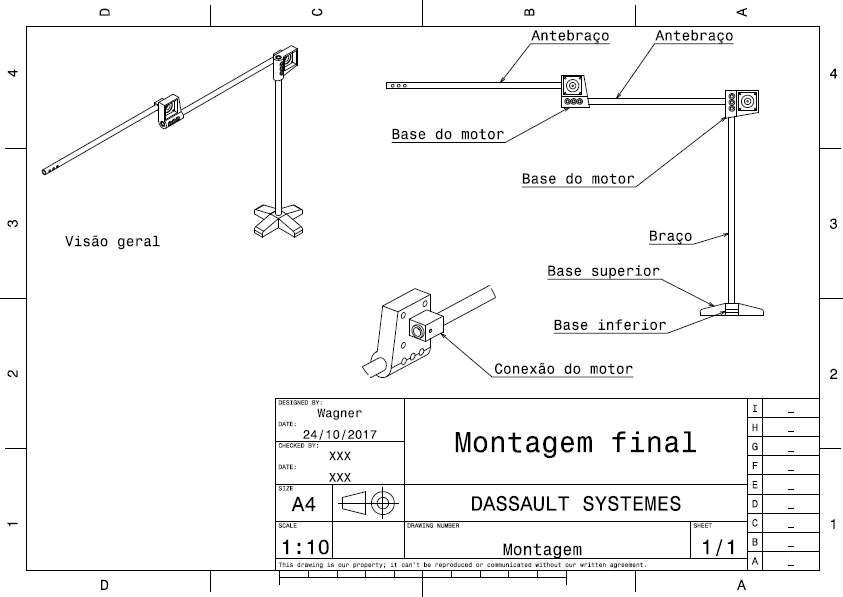
\includegraphics[keepaspectratio=true,scale=0.65]{figuras/braco_mecanico_7.png}
	\caption{Montagem final do braço mecânico após a integração de todas as peças constituintes.}
	\label{des_fig11}
\end{figure}
Já sobre o tipo do material que o braço seria composto, notou-se que os materiais de impressora 3D poderiam ser utilizados em várias partes do braço,por ser um material leve e barato, diminuindo, assim, os custos do projeto quando comparado a outros materiais. Os materiais que foram observados para o projeto são: o ABS (acrilonitrila butadieno estireno) e o PETG (politereftalato de etileno glicol)\cite{impressaofacil}.

O primeiro, ABS, é um material termoplástico derivado do petróleo amplamente utilizado na indústria e um dos principais e mais antigos materiais que vem sido utilizado na impressão 3D. Ele é rígido, bom, possui ótima resistência a impactos e possui uma leve flexibilidade quando comparada a outros materiais, permitindo uma pequena deformação ou flexão da peça, dependendo da sua geometria, o que é bom para peças que necessitem de encaixes em sua montagem; além de muito resistente a impactos,o material também é resistente a temperaturas altas. 

O segundo, PETG, é um material termoplástico derivado do petróleo, porém reciclável assim como o PET. Ele é utilizado na indústria há vários anos para diversas finalidades, mas, recentemente, tem sido usado na impressão 3D. Apresenta um aspecto transparente e brilhoso e produz peças tão resistentes a impactos quanto ao ABS, mas com flexibilidade e resistência ligeiramente superior a este. Resiste às altas temperaturas, mas não tanto como o ABS. O que o torna ideal para peças que precisem de transparência ou encaixes com maior flexibilidade, mantendo a alta resistência.
 
Para a escolha do material, foi feita uma tabela (figura \ref{des_fig12}) que permitisse enxergar melhor o material mais adequado. E ao analisar, foi perceptível que o material PETG é mais qualificado devido ao maior número de propriedades mais viáveis. No entanto, para a construção do braço 3D, optou-se pelo ABS devido a disponibilidades deste material ser maior.

\begin{figure}[H]
	\centering	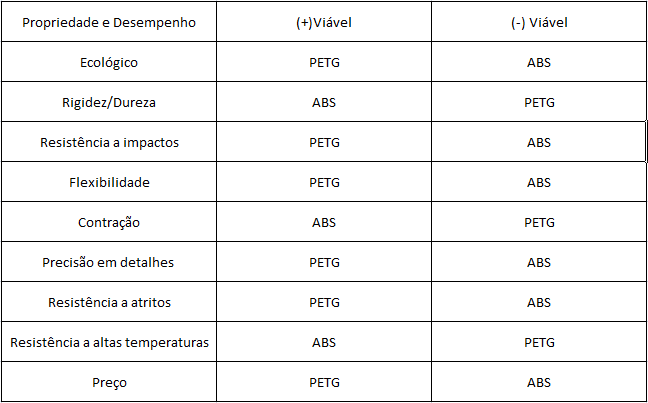
\includegraphics[keepaspectratio=true,scale=0.8]{figuras/tabela_braco_mecanico_1.png}
	\caption{Comparação entre PETG e ABS}
	\label{des_fig12}
\end{figure}
Outro material requisitado para compor a estrutura é o alumínio, pelo fato de ser altamente leve (possui uma densidade de apenas 2,7 g/cm$^3$, em comparação com uma densidade de 7,9 g/cm$^3$ para o aço), dúctil e por ter boa condutividade elétrica e térmica, além da alta resistência à corrosão em diversos ambientes. Sua dureza pode ainda ser elevada ao submetê-lo à formação de ligas e/ou processos de deformação plástica a frio\cite{william2013}.

Foram então escolhidos o ABS para constituir as juntas (com os encaixes para os motores e suas conexões com as hastes) e a liga 6061 T6 do alumínio para a fabricação da base, da haste fixa à base, do braço e do antebraço da estrutura. A liga fora escolhida pelo fato de apresentar boa resistência mecânica e viabilidade econômica, além de ser disponibilizada na forma de tubo \cite{bracomec}\cite{materialt6}.

Para verificar se os materiais escolhidos poderiam suportar as condições de carregamento impostas pelo pulso e pelo transdutor, foi efetuada a simulação do braço mecânico no software Ansys 18.1 com uma carga de 2 kg (aprox. 20N) posicionada na ponta do antebraço, de tal forma que todas as hastes permanecessem estendidas (pior caso possível de carregamento). O resultado pode ser visualizado na Figura \ref{des_fig13} a seguir:

\begin{figure}[H]
	\centering	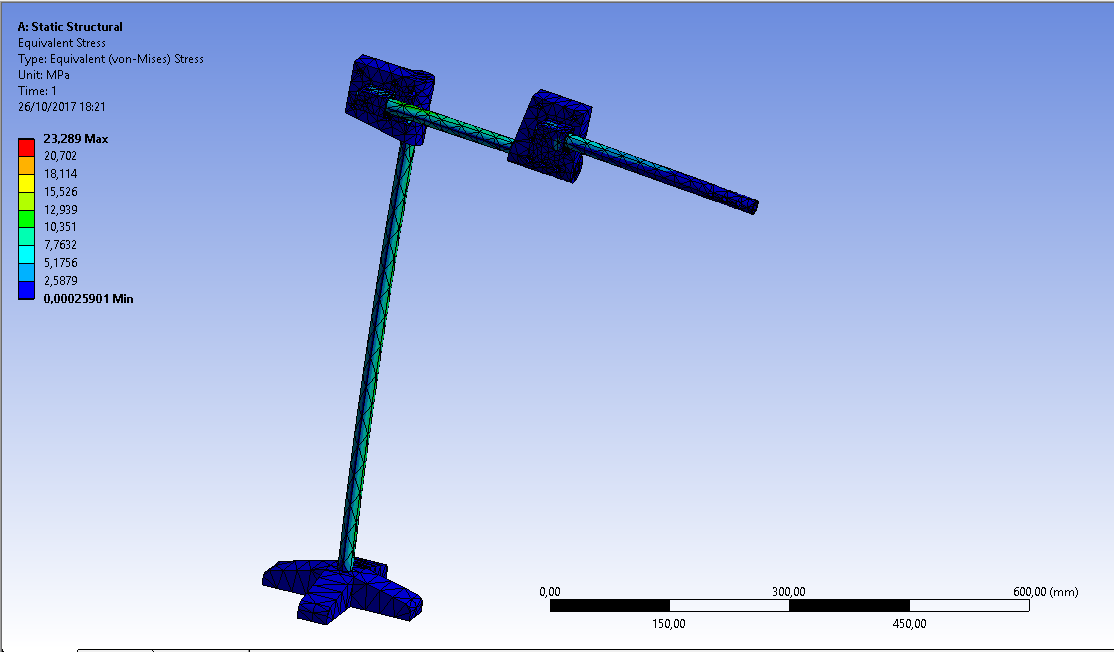
\includegraphics[keepaspectratio=true,scale=0.5]{figuras/braco_mecanico_8.png}
	\caption{Simulação de um carregamento de 2kg (20N) na ponta do antebraço do equipamento. }
	\label{des_fig13}
\end{figure}
A tensão máxima observada foi de 23,289 MPa, o que demonstra que o material submetido à carga máxima (liga de alumínio 6061 T6) suporta, com êxito, o carregamento imposto pelo pulso e pelo transdutor. Seu limite de escoamento é de 225 MPa \cite{materialt6}, mantendo-se na zona elástica do diagrama tensão-deformação. Para a fabricação da estrutura como um todo, deve haver atenção quanto às dimensões adotadas para não haver discrepâncias entre o resultado teórico simulado em computador e o experimental (real). 

Eletronicamente, o sistema escravo é composto por dois subsistemas eletrônicos distintos, sendo um o subsistema de controle do braço mecânico e o outro o sistema de ultrassom.
   
Para a movimentação do braço mecânico primeiramente foram analisados os dois melhores tipos de motores que podem ser utilizados para esta função, os servomotores e os motores de passo.

Os motores de passo possuem uma grande quantidade de pólos, geralmente entre 50 e 100, enquanto os servo possuem usualmente 4 a 12 pólos. O alto número de pólos permite que o motor de passo se mova de forma precisa e mais fácil entre cada pólo fazendo com que não necessite de um feedback de posição de um sensor externo. Devido ao seu design o motor de passo possui um torque constante de holding (segurar a posição) sem a necessidade de alimentação. A variedade de modelos, menor preço e disponibilidade no mercado são uma grande vantagem comparado com outros tipos de motores \cite{voss2008comprehensible}.

Para todas as suas vantagens, os motores de passo têm algumas limitações que podem causar importantes problemas de implementação e operação, dependendo da sua aplicação. Os motores de passo perdem uma quantidade significativa de torque quando eles se aproximam da velocidade máxima. A perda de 80\% do torque nominal em 90\% da velocidade máxima é típica. Os motores de passo também não são tão bons quanto os servos na aceleração de uma carga, além de problemas com vibração e ressonância.

Para aplicações em que alta velocidade e alto torque são necessários, servomotores se destacam. Servos além de possuírem velocidades bem maiores que os motores de passo, eles conseguem manter aproximadamente 90\% do torque mesmo em alto velocidade. Além disso servos motores não vibram ou sofrem de problemas de ressonância. Os servomotores são capazes de fornecer mais potência do que os motores de passo, mas exigem circuitos de acionamento muito mais complexos e feedback de posicionamento para um posicionamento preciso \cite{passovsservo}. 

Os servomotores também são muito mais caros do que os motores de passo e muitas vezes são mais difíceis de encontrar. Geralmente necessitam caixas de engrenagem, especialmente para operação com menor velocidade. O requisito para uma caixa de velocidades e um encoder de posição tornam os modelos de servos mais complexos mecanicamente e aumentam os requisitos de manutenção para o sistema. Além disso, os servo motores são mais caros do que os motores de passo antes de adicionar o custo de um codificador de posição \cite{passovsservo}.
               
Com base na aplicações necessárias do projeto e analisando as vantagens e desvantagens de cada tipo de motor, o motor de passo foi o escolhido.

Para a compra do motores e seus driver foi escolhido os produtos do grupo Grupo Neoyama que tem uma diversidade de modelos de motores de passo, drivers e fontes chaveadas no Brasil. Em específico os motores de passo da família Nema 23 e o driver D2282 devido a compatibilidade em relação ao torque máximo de holding e movimentação do braço. 

Na primeira tabela abaixo, figura \ref{des_fig14}, pode ser visto os diferentes modelos de motores de passos produzidos pela Neoyama e que cobrem os requisitos de cada parte do projeto que podem ser usados na estrutura do projeto, assim como a especificações de cada parte.  Na figura \ref{des_fig15} temo a tabela de especificação do driver escolhido para ser usado com a família Nema 23 de motores de passo.
\begin{figure}[H]
	\centering	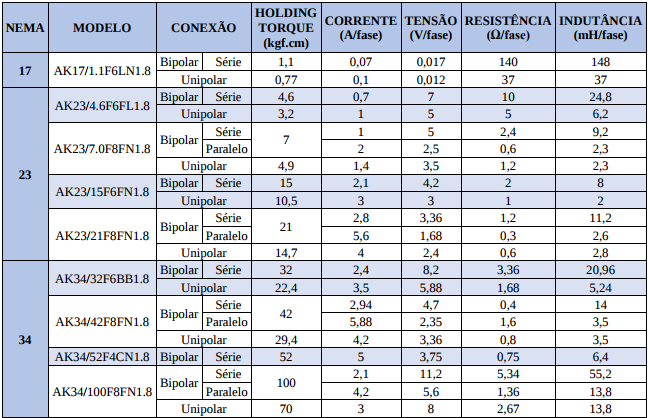
\includegraphics[keepaspectratio=true,scale=0.8]{figuras/tab1_des_eletronica.png}
	\caption{Especificações de motores de passo Nema \cite{passomotormanual}.}
	\label{des_fig14}
\end{figure}
\begin{figure}[H]
	\centering	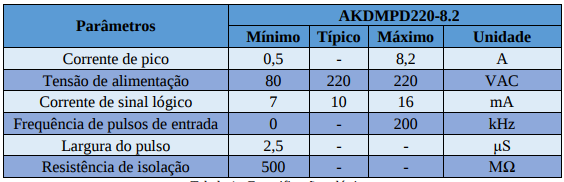
\includegraphics[keepaspectratio=true,scale=0.6]{figuras/tab3_des_eletronica.png}
	\caption{Especificação do driver D2282 (Modelo AKDMP8220-8.2A) \cite{drivermanual}}
	\label{des_fig15}
\end{figure}

A conexão entre o motor de passo Nema 23 e o driver é conforme o esquemático da figura \ref{des_fig16}.

\begin{figure}[H]
	\centering	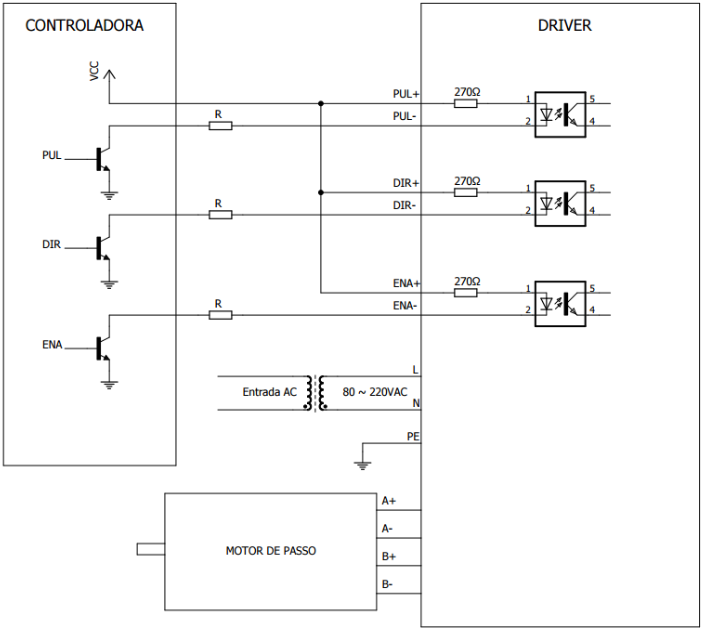
\includegraphics[keepaspectratio=true,scale=0.6]{figuras/conexao_driver_controlador_motorpasso.png}
	\caption{Esquemático da conexão entre driver, motor de passo e controlador \cite{drivermanual}}
	\label{des_fig16}
\end{figure}

Ao analisar a figura \ref{des_fig16} concluímos que o controle dos motores de passo é feito da seguinte forma: 

\begin{enumerate}[noitemsep]
\item O controlador, Arduino, recebe os sinais advindos no sistema principal via cabo usb no formato serial;
\item Arduino processa os sinais recebidos e envia os sinais de controle processados para cada um dos drivers dos motores de passo;
\item O driver, que é alimentado via tomada por necessitar de uma fonte 220ac, recebe os sinais advindos do Arduino, processa, e manda os sinais de movimento para o motor de passo.
\end{enumerate}


Para o controle dos motores será utilizado o Arduino Due, figura \ref{ard_due}, devido a necessidade de utilizar um chip ARM para processar os sinais advindos do sistema de controle para os comandos para cada um dos motores de passo, além da necessidade de uma porta USB que envia os sinais seriais do computador para o Arduino e de uma quantidade maior de pinos de conexão para os vários motores existentes. Abaixo temos as especificações do Arduino Due \cite{arduinodue}:

\begin{itemize}[noitemsep]
\item Microcontrolador:  	AT91SAM3X8E
\item Tensão de operação (nível lógico): 3.3V
\item Tensão de entrada (recomendada): 7-12V
\item Tensão de entrada (limites): 6-16V
\item Pinos digitais I/O: 54, dos quais 12 podem ser saídas PWM
\item Pinos de entrada analógica: 12
\item Pinos de saída analógica: 2 (DAC)
\item Corrente contínua no pino I/O: 130 mA
\item Corrente contínua no pino de 3.3V: 800 mA
\item Corrente contínua no pino de 5V: 800 mA
\item Memória Flash: 512KB (dos quais 2KB são utilizados pelo bootloader)
\item SRAM: 96KB
\item Velocidade de clock : 84 MHz
\item Dimensões:  101.52mm x 53.3mm
\begin{figure}[H]
	\centering	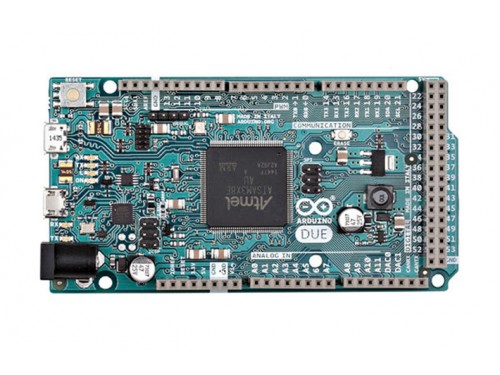
\includegraphics[keepaspectratio=true,scale=0.8]{figuras/ard_due.jpg}
	\caption{Arduino DUE}
	\label{ard_due}
\end{figure}
\end{itemize}

Para programação do Arduino será utilizada principalmente a biblioteca stepper.h, nativa ao software IDE do arduino.

A biblioteca stepper.h permite controlar motores de passo unipolares e bipolares . Um driver apropriado deve ser utilizado a velocidade pode ser controlada. Também é possível girar o motor umas quantidade de passos desejada. Na figura \ref{des_fig17} se tem um esboço básico demonstrando como seria o controle de um motor de passo simples.

\begin{figure}[H]
	\centering	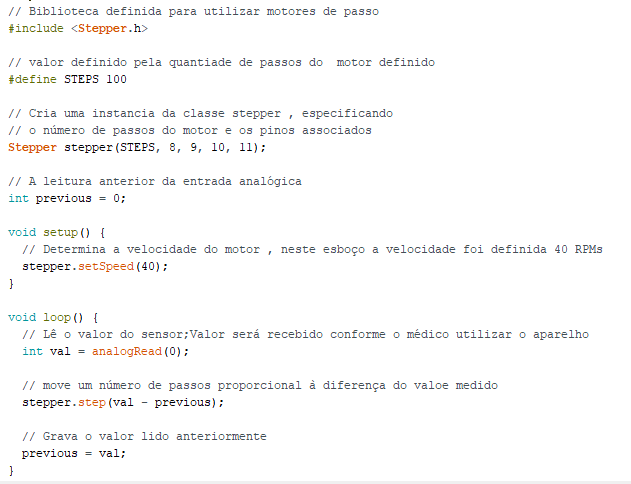
\includegraphics[keepaspectratio=true,scale=0.6]{figuras/figura_stepper.png}
	\caption{Esboço do código para controle de um motor de passo}
	\label{des_fig17}
\end{figure}

Um sinal é a representação de uma variável, física ou não, dependente que varia em função de uma variável dependente ou independente, quando um ou mais sinais são processados ou modificados por uma ou mais entidades estas são consideradas sistemas \cite{alanoppenheim}.

Um sistema pode ser classificado como causal ou não-causal, linear ou não-linear e variante ou não no tempo, dentre outras denominações. O sistema aqui abordado processa sinais (coordenadas) compara com as coordenadas do transdutor, modifica a posição do transdutor com o auxílio de motores, aproveitando a característica das juntas que funcionam como rótulas permitindo a movimentação de forma independente entre os elementos lineares ou elos.

Da forma como foi concebido o sistema é causal pois depende apenas da posição informada pelo sistema de comunicação e da posição atual do transdutor, necessitando assim armazenar a posição recebida e subtrair da posição do transdutor para poder determinar o quanto deve se deslocar para que o transdutor permaneça na posição desejada. Desta forma:
\begin{align*}
y(n) = x(n) - x(n-1)
\end{align*}
Onde:\\
$\cdot$ x(n) é a posição informada.\\
$\cdot$ x(n-1) é a posição do transdutor.\\
$\cdot$ y(n) é a quantidade de espaço em que o transdutor deve ser movimentado para permanecer nas coordenadas informadas.

Para movimentação em cada eixo será criado um procedimento. O algoritmo é representado, de forma simples, através da figura \ref{des_fig18}.

\begin{figure}[H]
	\centering	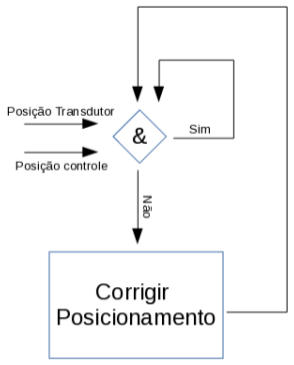
\includegraphics[keepaspectratio=true,scale=0.6]{figuras/algoritmo_motor.png}
	\caption{Fluxograma do algoritmo para movimentação dos eixos}
	\label{des_fig18}
\end{figure}

O segundo subsistema eletrônico do sistema escravo, o sistema de ultrassom, foi trabalhado com base no exigido pelo projeto. Dessa forma, o sistema de ultrassom escolhido deve ter como especificação mínima uma saída de vídeo, VGA ou S-VIDEO, ser portátil e ser compatível com transdutores lineares e transdutores convexos. Essas características mínimas são com base na limitação para exames na região do torso humano e a necessidade de transmissão das imagens da tela do ultrassom para um computador com conexão de internet. Com base nestas características, tem-se a comparação, de alguns modelos existentes no mercado, presente na tabela \ref{tabela-comp-ultrassom}.

\begin{center}
\begin{table}[H]
\caption{Comparação entre modelos de ultrassom portátil (\cite{philipscx50}, \cite{samsungsonou6}, \cite{samsunghm70a}, \cite{gevenue40}, \cite{sonoscapea6})}
\label{tabela-comp-ultrassom}
\resizebox{\textwidth}{!}{
\begin{tabular}{|
>{\columncolor[HTML]{009901}}l |
>{\columncolor[HTML]{009901}}c |
>{\columncolor[HTML]{38FFF8}}c |
>{\columncolor[HTML]{F5DEB3}}c |
>{\columncolor[HTML]{F5DEB3}}c |
>{\columncolor[HTML]{F5DEB3}}c |
>{\columncolor[HTML]{F5DEB3}}c |
>{\columncolor[HTML]{F5DEB3}}c |}
\hline
\multicolumn{2}{|l|}{\cellcolor[HTML]{FFFFFF}{\color[HTML]{FFFFFF} }}                                                                                                           & \multicolumn{6}{c|}{\cellcolor[HTML]{3531FF}{\color[HTML]{FFFFFF} Aparelhos de Ultrassonografia}}                                                                                                                                                                                                                                                                                                                                                                                                                                                                          \\ \cline{3-8} 
\multicolumn{2}{|l|}{\multirow{-2}{*}{\cellcolor[HTML]{FFFFFF}{\color[HTML]{FFFFFF} }}}                                                                                         & {\color[HTML]{000000} Peso} & \cellcolor[HTML]{3531FF}{\color[HTML]{FFFFFF} \begin{tabular}[c]{@{}c@{}}Philips \\ CX50\end{tabular}} & \cellcolor[HTML]{3531FF}{\color[HTML]{FFFFFF} \begin{tabular}[c]{@{}c@{}}Venue \\ 40\end{tabular}} & \cellcolor[HTML]{3531FF}{\color[HTML]{FFFFFF} \begin{tabular}[c]{@{}c@{}}SonoScape \\ A6\end{tabular}} & \cellcolor[HTML]{3531FF}{\color[HTML]{FFFFFF} \begin{tabular}[c]{@{}c@{}}Samsung \\ MySono U6\end{tabular}} & \cellcolor[HTML]{3531FF}{\color[HTML]{FFFFFF} \begin{tabular}[c]{@{}c@{}}Samsung \\ HM70A\end{tabular}} \\ \hline
\cellcolor[HTML]{009901}{\color[HTML]{FFFFFF} }                       & {\color[HTML]{FFFFFF} Saída de Vídeo VGA}                                                               & 6                           & {\color[HTML]{000000} S}                                                                               & {\color[HTML]{000000} S}                                                                           & {\color[HTML]{000000} 0}                                                                               & {\color[HTML]{000000} S}                                                                                    & {\color[HTML]{000000} S}                                                                                \\ \cline{2-8} 
\cellcolor[HTML]{009901}{\color[HTML]{FFFFFF} }                       & {\color[HTML]{FFFFFF} Portabilidade}                                                                    & 5                           & {\color[HTML]{000000} +}                                                                               & {\color[HTML]{000000} S}                                                                           & {\color[HTML]{000000} 0}                                                                               & {\color[HTML]{000000} -}                                                                                    & {\color[HTML]{000000} -}                                                                                \\ \cline{2-8} 
\cellcolor[HTML]{009901}{\color[HTML]{FFFFFF} }                       & {\color[HTML]{FFFFFF} Qualidade da imagem}                                                              & 4                           & {\color[HTML]{000000} +}                                                                               & {\color[HTML]{000000} -}                                                                           & {\color[HTML]{000000} 0}                                                                               & {\color[HTML]{000000} +}                                                                                    & {\color[HTML]{000000} +}                                                                                \\ \cline{2-8} 
\cellcolor[HTML]{009901}{\color[HTML]{FFFFFF} }                       & {\color[HTML]{FFFFFF} \begin{tabular}[c]{@{}c@{}}Quantidade de \\ transdutores suportados\end{tabular}} & 1                           & {\color[HTML]{000000} +}                                                                               & {\color[HTML]{000000} +}                                                                           & {\color[HTML]{000000} 0}                                                                               & {\color[HTML]{000000} +}                                                                                    & {\color[HTML]{000000} +}                                                                                \\ \cline{2-8} 
\cellcolor[HTML]{009901}{\color[HTML]{FFFFFF} }                       & {\color[HTML]{FFFFFF} \begin{tabular}[c]{@{}c@{}}Aplicações suportadas\\ pelo software\end{tabular}}    & 2                           & {\color[HTML]{000000} +}                                                                               & {\color[HTML]{000000} +}                                                                           & {\color[HTML]{000000} 0}                                                                               & {\color[HTML]{000000} +}                                                                                    & {\color[HTML]{000000} +}                                                                                \\ \cline{2-8} 
\cellcolor[HTML]{009901}{\color[HTML]{FFFFFF} }                       & {\color[HTML]{FFFFFF} \begin{tabular}[c]{@{}c@{}}Tempo de garantida \\ do fornecedor\end{tabular}}      & 3                           & {\color[HTML]{000000} -}                                                                               & {\color[HTML]{000000} +}                                                                           & {\color[HTML]{000000} 0}                                                                               & {\color[HTML]{000000} S}                                                                                    & {\color[HTML]{000000} S}                                                                                \\ \cline{2-8} 
\multirow{-7}{*}{\cellcolor[HTML]{009901}\rot{{\color[HTML]{FFFFFF} Critérios}}} & {\color[HTML]{FFFFFF} Preço}                                                                            & 10                          & {\color[HTML]{000000} -}                                                                               & {\color[HTML]{000000} -}                                                                           & {\color[HTML]{000000} 0}                                                                               & {\color[HTML]{000000} -}                                                                                    & {\color[HTML]{000000} -}                                                                                \\ \hline
\multicolumn{3}{|c|}{\cellcolor[HTML]{DA70D6}{\color[HTML]{343434} Peso Total}}                                                                                                                               & \cellcolor[HTML]{DA70D6}{\color[HTML]{343434} -1}                                                      & \cellcolor[HTML]{DA70D6}{\color[HTML]{343434} -8}                                                  & \cellcolor[HTML]{DA70D6}{\color[HTML]{343434} 0}                                                       & \cellcolor[HTML]{DA70D6}{\color[HTML]{343434} -8}                                                           & \cellcolor[HTML]{DA70D6}{\color[HTML]{343434} -8}                                                       \\ \hline
\end{tabular}}
\end{table}
\end{center}

Analisando os dados fornecidos pela tabela \ref{tabela-comp-ultrassom}, pode-se concluir que a melhor opção, levando em consideração os critérios, é o Sonoscape A6, figura \ref{des_fig19}. Este sistema suporta vários tipos de transdutores, incluindo um linear e dois convexos, para realização dos mais variados tipos de exame. Integrado ao seu sistema também existe alguns recursos interessantes como fórmulas médicas para analise das imagens de ultrasom, entrada de cabo de internet por onde pode ser configurado um servidor DICOM 3.0 (recebe as imagens advindas do sistema se necessário), duas entradas usb para transferência local das imagens do exame se o paciente necessitar. O valor médio para esse produto varia entre \$ 4,250.00 e \$ 6,499.00 \cite{sonoscapea6}.
\begin{figure}[H]
	\centering	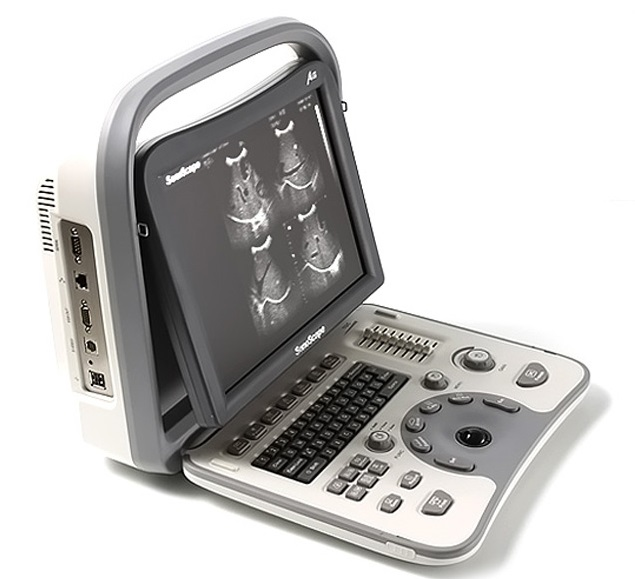
\includegraphics[keepaspectratio=true,scale=0.35]{figuras/sonoscapea6.jpg}
	\caption{Sistema de ultrassonografia Sonoscape A6}
	\label{des_fig19}
\end{figure}
O transdutor linear escolhido para uso neste projeto é o Linear Array L745 (figura \ref{des_fig20}), 128 elementos e frequência doppler entre 5-12 MHz,  e o transdutor convexo escolhido é o Convex Array C351 (figura \ref{des_fig21}), 128 elementos e frequência doppler entre 3-8Mhz, sendo este último modelo indicado para uso em adultos. O preço para cada unidade desses transdutores é de aproximadamente \$ 1,800.00.

\begin{figure}[H]
\centering
\begin{subfigure}{.5\textwidth}
  \centering
  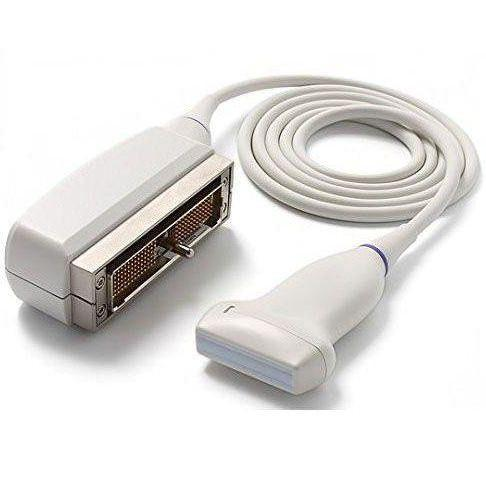
\includegraphics[width=.8\linewidth]{figuras/sonoscape-linear-array-transducer-l745_grande.jpg}
  \caption{Transdutor linear L745}
  \label{des_fig20}
\end{subfigure}%
\begin{subfigure}{.5\textwidth}
  \centering
  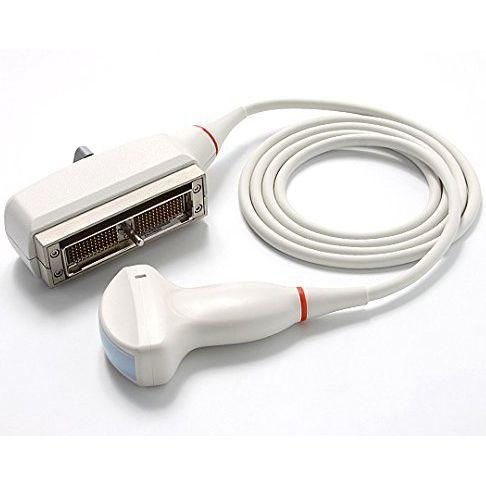
\includegraphics[width=.8\linewidth]{figuras/sonoscape-convex-array-transducer-c351_grande.jpg}
  \caption{Transdutor convexo C351}
  \label{des_fig21}
\end{subfigure}
\caption{Transdutores selecionados para o projeto}
\label{comb_2fig}
\end{figure}

Para transmissão dos dados das imagens do aparelho de ultrassom para o computador, utilizando a porta VGA, deve-se utilizar um dispositivo de captura de vídeo. Este aparelho tem função de receber as imagens advindas da porta VGA e converter em  sinais de imagem serial (USB) transmitidas para o computador na codificação MPEG4/H.264. Tanto a codificação MPEG4 quanto a H.264 são suportadas pelos sistemas operacionais Windows quanto Ubuntu do computador que recebe os sinais de imagem.

Para este projeto foi escolhido o USB 3.0 Video Capture Device da empresa StarTech, figura \ref{des_fig22}. As principais características deste produto é suportar imagens até a qualidade 1080p com taxa de atualização de 60fps e entrada de vídeo VGA. A saída para este aparelho é uma porta USB 3.0 que é conectada a um computador compatível com a tecnologia USB 3.0, conforme especificação do fabricante não funciona em aparelhos com USB 2.0 ou inferior.
\begin{figure}[H]
	\centering	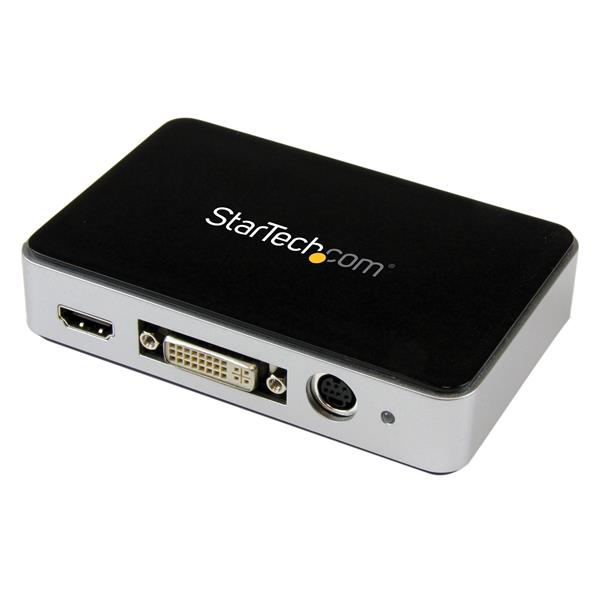
\includegraphics[keepaspectratio=true,scale=0.35]{figuras/startech.jpg}
	\caption{Dispositivo de captura de vídeo StarTech USB 3.0}
	\label{des_fig22}
\end{figure}

Como último componente para parte eletrônica do sistema escravo temos o computador. Para escolha dele levamos em considerações os requisitos exigidos pelos outros sistemas descritos anteriormente, portabilidade e, principalmente, preço. Na tabela \ref{comp_computadores}, a seguir, temos uma comparação entre alguns modelos de notebook encontrados no mercado.

\begin{center}
\begin{table}[H]
\caption{Comparação entre modelos de notebook (\cite{notebook1}, \cite{notebook2}, \cite{notebook5}, \cite{notebook3}, \cite{notebook4})}
\label{comp_computadores}
\resizebox{\textwidth}{!}{
\begin{tabular}{|
>{\columncolor[HTML]{009901}}l |
>{\columncolor[HTML]{009901}}c |
>{\columncolor[HTML]{38FFF8}}c |
>{\columncolor[HTML]{F5DEB3}}c |
>{\columncolor[HTML]{F5DEB3}}c |
>{\columncolor[HTML]{F5DEB3}}c |
>{\columncolor[HTML]{F5DEB3}}c |
>{\columncolor[HTML]{F5DEB3}}c |}
\hline
\multicolumn{2}{|l|}{\cellcolor[HTML]{FFFFFF}{\color[HTML]{FFFFFF} }}                                                                                                           & \multicolumn{6}{c|}{\cellcolor[HTML]{3531FF}{\color[HTML]{FFFFFF} Notebooks}}                                                                                                                                                                                                                                                                                                                                                                                                                                                                          \\ \cline{3-8} 
\multicolumn{2}{|l|}{\multirow{-2}{*}{\cellcolor[HTML]{FFFFFF}{\color[HTML]{FFFFFF} }}}                                                                                         & {\color[HTML]{000000} Peso} & \cellcolor[HTML]{3531FF}{\color[HTML]{FFFFFF} \begin{tabular}[c]{@{}c@{}}Acer \\ Aspire E \end{tabular}} & \cellcolor[HTML]{3531FF}{\color[HTML]{FFFFFF} \begin{tabular}[c]{@{}c@{}}Acer \\ Aspire 5\end{tabular}} & \cellcolor[HTML]{3531FF}{\color[HTML]{FFFFFF} \begin{tabular}[c]{@{}c@{}}HP Compaq \\ Presario\end{tabular}} & \cellcolor[HTML]{3531FF}{\color[HTML]{FFFFFF} \begin{tabular}[c]{@{}c@{}}Lenovo \\ Ideapad 320\end{tabular}} & \cellcolor[HTML]{3531FF}{\color[HTML]{FFFFFF} \begin{tabular}[c]{@{}c@{}}Asus \\ Vivobook Flip\end{tabular}} \\ \hline
\cellcolor[HTML]{009901}{\color[HTML]{FFFFFF} }                       & {\color[HTML]{FFFFFF} \begin{tabular}[c]{@{}c@{}}Quantidade de \\ portas USB 3.0 \end{tabular}}                                                                 & 6                           & {\color[HTML]{000000} S}                                                                               & {\color[HTML]{000000} +}                                                                           & {\color[HTML]{000000} 0}                                                                               & {\color[HTML]{000000} +}                                                                                    & {\color[HTML]{000000} +}                                                                                \\ \cline{2-8} 
\cellcolor[HTML]{009901}{\color[HTML]{FFFFFF} }                       & {\color[HTML]{FFFFFF} \begin{tabular}[c]{@{}c@{}}Quantidade de \\ portas USB 2.0 \end{tabular}}                                                                 & 5                           & {\color[HTML]{000000} S}                                                                               & {\color[HTML]{000000} -}                                                                           & {\color[HTML]{000000} 0}                                                                               & {\color[HTML]{000000} -}                                                                                    & {\color[HTML]{000000} +}                                                                                \\ \cline{2-8} 
\cellcolor[HTML]{009901}{\color[HTML]{FFFFFF} }                       & {\color[HTML]{FFFFFF} Entrada de internet}                                                              & 4                           & {\color[HTML]{000000} S}                                                                               & {\color[HTML]{000000} S}                                                                           & {\color[HTML]{000000} 0}                                                                               & {\color[HTML]{000000} S}                                                                                    & {\color[HTML]{000000} S}                                                                                \\ \cline{2-8} 
\cellcolor[HTML]{009901}{\color[HTML]{FFFFFF} }                       & {\color[HTML]{FFFFFF} \begin{tabular}[c]{@{}c@{}}Velocidade de \\processamento \end{tabular}} & 1                           & {\color[HTML]{000000} +}                                                                               & {\color[HTML]{000000} +}                                                                           & {\color[HTML]{000000} 0}                                                                               & {\color[HTML]{000000} +}                                                                                    & {\color[HTML]{000000} +}                                                                                \\ \cline{2-8} 
\cellcolor[HTML]{009901}{\color[HTML]{FFFFFF} }                       & {\color[HTML]{FFFFFF} \begin{tabular}[c]{@{}c@{}}Espaço de \\armazenamento interno\end{tabular}}    & 2                           & {\color[HTML]{000000} +}                                                                               & {\color[HTML]{000000} +}                                                                           & {\color[HTML]{000000} 0}                                                                               & {\color[HTML]{000000} +}                                                                                    & {\color[HTML]{000000} +}                                                                                \\ \cline{2-8} 
\cellcolor[HTML]{009901}{\color[HTML]{FFFFFF} }                       & {\color[HTML]{FFFFFF} \begin{tabular}[c]{@{}c@{}}Tempo de garantida \\ do fornecedor\end{tabular}}      & 3                           & {\color[HTML]{000000} S}                                                                               & {\color[HTML]{000000} S}                                                                           & {\color[HTML]{000000} 0}                                                                               & {\color[HTML]{000000} S}                                                                                    & {\color[HTML]{000000} S}                                                                                \\ \cline{2-8} 
\multirow{-7}{*}{\cellcolor[HTML]{009901}\rot{{\color[HTML]{FFFFFF} Critérios}}} & {\color[HTML]{FFFFFF} Preço}                                                                            & 7                          & {\color[HTML]{000000} +}                                                                               & {\color[HTML]{000000} -}                                                                           & {\color[HTML]{000000} 0}                                                                               & {\color[HTML]{000000} S}                                                                                    & {\color[HTML]{000000} -}                                                                                \\ \hline
\multicolumn{3}{|c|}{\cellcolor[HTML]{DA70D6}{\color[HTML]{343434} Peso Total}}                                                                                                                               & \cellcolor[HTML]{DA70D6}{\color[HTML]{343434} 10}                                                      & \cellcolor[HTML]{DA70D6}{\color[HTML]{343434} -9}                                                  & \cellcolor[HTML]{DA70D6}{\color[HTML]{343434} 0}                                                       & \cellcolor[HTML]{DA70D6}{\color[HTML]{343434} -2}                                                           & \cellcolor[HTML]{DA70D6}{\color[HTML]{343434} 7}                                                       \\ \hline
\end{tabular}}
\end{table}
\end{center}

Analisando os pesos totais obtidos por cada produto, tabela \ref{comp_computadores}, temos como melhor escolha o notebook Acer Aspire E Series ES1-572, figura \ref{acer_note}. A especificação mais importante que está incluida nesse modelo é incluir 2 conexões USB 2.0, 1 conexão USB 3.0 e entrada de internet RJ-45 tipo Gigabit 10/100/1000. O preço médio, conforme data deste relátório, é de R\$ 1,700.00. A seguir temos algumas especificações deste produto \cite{notebook1}:

\begin{itemize}[noitemsep]
\item Modelo: NX.GMFAL.005
\item Processador: i3-7100U (Frequência entre 1.1 Ghz e 2.4 Ghz na função turbo)
\item Tela: 15.6" HD LED LCD - Resolução 1920x1080
\item Memória ram: 4GB 1600Mhz DDR4
\item Placa de rede: Wireless padrão - 802.11b/g/n
\item Armazenamento: HD de 1TB (5400 RPM)
\item Bateria: Lítio prismático - 3220 mAh
\item Sistema operacional: Windows 10
\item Peso: 2,4 kg
\item Dimensões: 381.8 x 258 x 24.6 mm
\begin{figure}[H]
	\centering	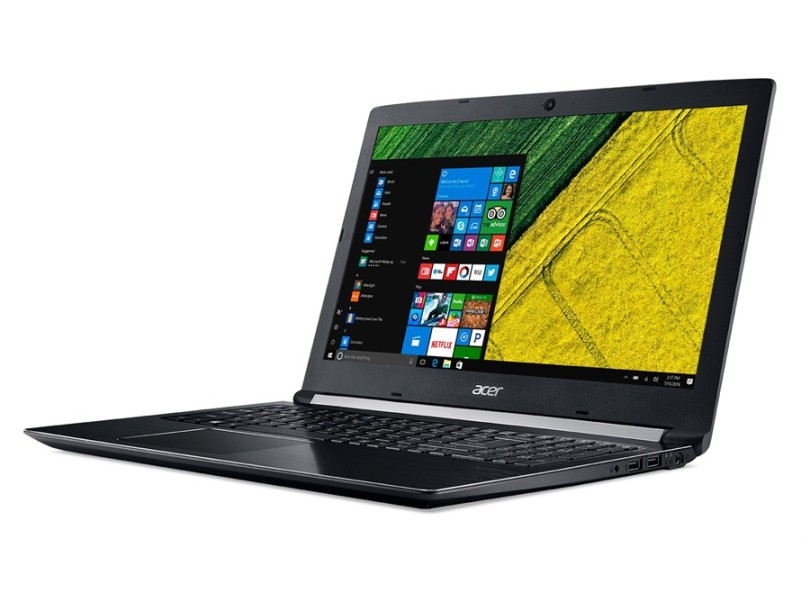
\includegraphics[keepaspectratio=true,scale=0.3]{figuras/acer_note.jpg}
	\caption{Notebook Acer Aspire E Series ES1-572 \cite{notebook1}}
	\label{acer_note}
\end{figure}
\end{itemize}

A forma de comunicação Arduino/PC escolhida foi a USART (Universal Synchronous Asynchrous Receiver Transmitter). Essa forma de comunicação se caracteriza, principalmente, por ser Full-Duplex (Registradores de recepção e transmissão independentes) e pode trabalhar de forma síncrona ou assíncrona, além de ser também uma forma bastante flexível de comunicação serial.

A USART é uma abordagem simples de comunicação, que utiliza de 3 fios (Rx, Tx e GND) e que pode ser facilmente controlada. Rx e Tx são os fios que irão nos pinos RX e Tx do microcontrolador para fazer a recepção (Rx) e transmissão (Tx) dos dados. Nos arduinos com porta USB/mUSA integrados, tem-se a opção de transmitir os mesmos dados destes 3 fios via USB. O arduino já possui bibliotecas nativas para a utilização deste protocolo e no computador basta configurar a porta serial para a recepção e envio de dados.

Utilizando um oscilador de 16MHz no microcontrolador pode-se alcançar uma taxa de transmissão de até 2Mbps, podendo chegar a 2.5Mbps caso seja utilizado um oscilador de 20MHz.

O frame enviado por este protocolo é composto de 1 bit de início, de 5 a 9 bits de dados, 1 ou nenhum bit de paridade e 1 ou 2 bits de parada. No final da transmissão de um frame pode-se transmitir outro frame ou se pode ficar em estado de iddle (nível lógico alto). Caso trabalhe em modo síncrono os bits de início e parada não serão necessários.

Para alimentar energeticamente o braço, como falado anteriormente, será utilizada tomada de 110V ou 220V, como fonte primária de energia. Entretanto, para segurança do paciente, caso essa fonte energética falhe, foi pensada uma segunda fonte energética, a bateria Moura chumbo ácido 12 V, que foi descrita anteriormente.

Contudo, foi pensado também, para o braço, uma placa fotovoltaica que será utilizada como opção de transmissão de energia, sendo necessária apenas para suprir áreas com inconstâncias no sistema elétrico ou sem energia e que possua radiação solar em abundância. Ou seja, essa placa é um sistema de segurança para que o sistema não pare durante o procedimento de ultrassom.

O sistema de placa fotovoltaica foi escolhido devido a sua eficiência, jpa que há uma grande incidência solar em todo o Brasil. Porém, não é indicado para regiões úmidas e com altos índices pluviométricos, pois a umidade afeta muito a eficiência da placa solar. Abaixo está presente a figura \ref{des_fig23},que mostra a média anual de incidência de radiação solar no Brasil, de acordo com o Portal Solar.

\begin{figure}[H]
	\centering	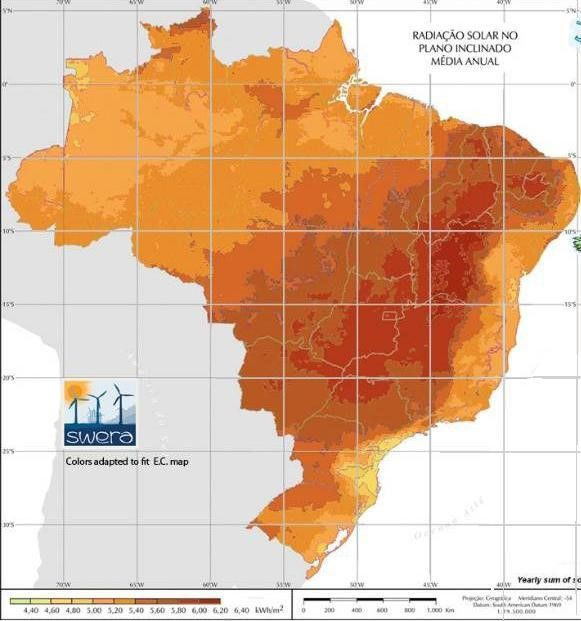
\includegraphics[keepaspectratio=true,scale=0.57]{figuras/mapasolar_brasil.jpg}
	\caption{Média anual de incidência de radiação solar no Brasil}
	\label{des_fig23}
\end{figure}

A placa fotovoltaica é uma placa de silício policristalino, sendo suas vantagens uma vida útil maior que 30 anos, possuindo uma garantia de 25 anos e ser barato; entretanto possui desvantagens como menor eficiência, menos watts por hora por m$^2$. Mas, por ser um sistema de supressão, a eficiência dessa placa é suficiente para atender as necessidades do produto \cite{portalso1}.

Estruturalmente, a placa possui uma forma quadrada de 10 cm x 10 cm e a eficiência de 13 a 16,5\%. O tamanho da placa é a que melhor atende o braço mecânico e ela possui uma cor azul com antirreflexo, que melhora um pouco a sua eficiência. A figura \ref{des_fig24} mostra essa placa.

\begin{figure}[H]
	\centering	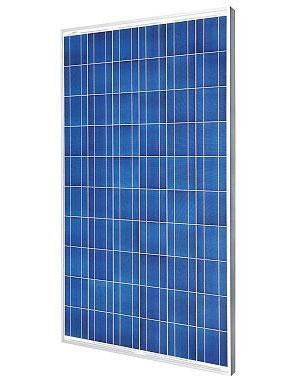
\includegraphics[keepaspectratio=true,scale=0.7]{figuras/placafotovoltaica_brasil.jpg}
	\caption{Placa de Silício Policristalino}
	\label{des_fig24}
\end{figure}

O painel solar produz energia elétrica em corrente contínua; o inversor solar converte a energia em corrente alternada, deixando-a pronta para ser usada. Essa energia produzida pelas células fotovoltaicas nos painéis é transformada pelo inversor e será armazenada na bateria, que deixará a energia pronto para consumo.

\section{COMUNICAÇÃO ENTRE OS SISTEMAS}

A comunicação entre o sistema principal e o sistema escravo, como já descrito, será feita por meio de transmissão de comandos e imagens entre as unidades, utilizando a arquitetura de soquetes de internet. 

    Como mostrado na figura 3, a unidade principal transmite os dados de movimento, o servidor analisa e transmite os comandos para a unidade escrava (unidade de ultrassom), essa unidade transmite as imagens geradas para o servidor, que encaminha para a unidade de controle, que recebe essas imagens.
    
    A linguagem escolhida foi Python e se deu pelo fato de ser uma linguagem de alto-nível com um bom suporte a pacotes e com um grande número de frameworks e bibliotecas evoluídas para o desenvolvimento web, como por exemplo: Django, Flask e Tornado. Esse tipo de suporte torna o desenvolvimento mais produtivo e evita retrabalho. Além disso, de acordo com uma pesquisa feita pela IEEE \cite{IEEElang}, o python é hoje a linguagem de programação mais popular, o que significa que desenvolver e manter esse serviço não será problema.
    
    Foi desenvolvido um código, que implementa a transmissão de vídeo utilizando o python. O código foi dividido em dois servers, um que é da captura da imagem do ultrassom e transmite para o segundo server; esse interpreta e expõe a imagem na tela do usuário (o médico).
    
    O server de transmissão utiliza a biblioteca pygame para acessar a câmera conectada, logo após a biblioteca socket cuida de estabelecer a conexão com o cliente que vai receber o vídeo. Concluída a conexão o server de captura começa a capturar várias fotos seguidas e enviá-las ao cliente. As figuras \ref{soft_1}, \ref{soft_2} e \ref{soft_3} a seguir mostram as bibliotecas, a configuração de socket e a captura e transmissão de imagem.

\begin{figure}[H]
	\centering	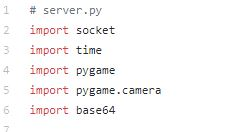
\includegraphics[keepaspectratio=true,scale=1]{figuras/2_0_bibliotecas_server_transm.jpg}
	\caption{Bibliotecas do servidor de transmissão}
	\label{soft_1}
\end{figure}

\begin{figure}[H]
	\centering	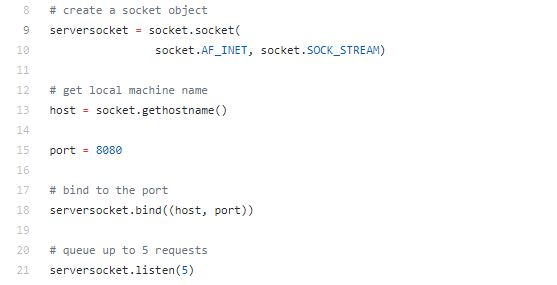
\includegraphics[keepaspectratio=true,scale=1]{figuras/2_1_socket_server_transm.jpg}
	\caption{Configuração de socket}
	\label{soft_2}
\end{figure}

\begin{figure}[H]
	\centering	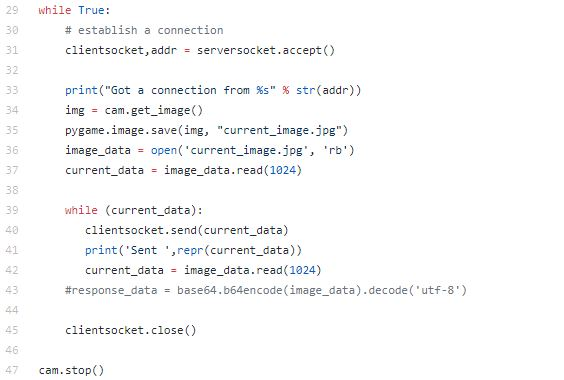
\includegraphics[keepaspectratio=true,scale=1]{figuras/2_2_captura_server_transm.jpg}
	\caption{Captura e transmissão de imagem}
	\label{soft_3}
\end{figure}

O servidor cliente (do médico) também utiliza da biblioteca pygame para primeiramente definir uma janela de exibição para o vídeo, após estabelecer a conexão via socket utilizando a biblioteca específica o cliente carrega cada imagem recebida, através da conexão, na janela do cliente utilizando o método image.load da biblioteca pygame. As figuras \ref{soft_4}, \ref{soft_5} e \ref{soft_6} mostram as bibliotecas do servidor cliente, o código que define a tela para transmissão do vídeo e o código que recebe as imagens transmitidas.

\begin{figure}[H]
	\centering	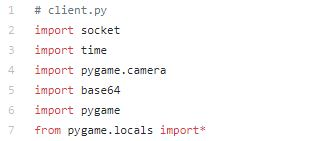
\includegraphics[keepaspectratio=true,scale=1]{figuras/2_3_bibliotecas_client.jpg}
	\caption{bibliotecas do servidor cliente}
	\label{soft_4}
\end{figure}

\begin{figure}[H]
	\centering	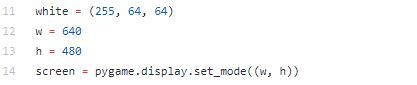
\includegraphics[keepaspectratio=true,scale=1]{figuras/2_4_tela_cliente.jpg}
	\caption{Definição da tela para transmissão do vídeo}
	\label{soft_5}
\end{figure}

\begin{figure}[H]
	\centering	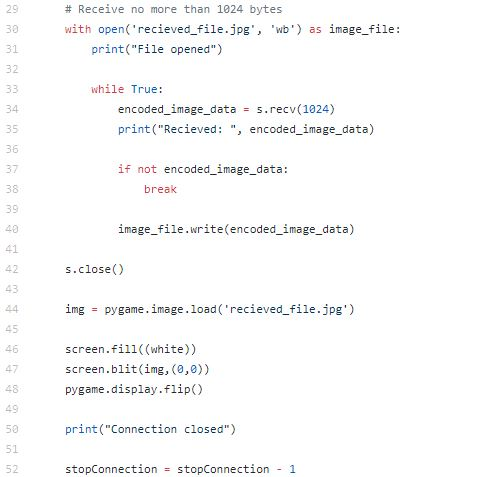
\includegraphics[keepaspectratio=true,scale=1]{figuras/2_5_carregar_cliente.jpg}
	\caption{Recepção das imagens transmitidas}
	\label{soft_6}
\end{figure}

O servidor de transmissão e o servidor cliente podem ser encontrados, respectivamente, nos links: \hyperlink{Servidor de transmissão}{https://github.com/PI1-Turma-E/liveImag} e \hyperlink{Servidor client}{https://github.com/PI1-Turma-E/liveClient}.

Além disso, foram desenvolvidos dois protótipos de alta fidelidade, o primeiro correspondente a tela que o médico terá acesso ao realizar os exames e o segundo referente a tela que o paciente irá visualizar durante o exame.

Na tela do médico, ele irá visualizar na parte superior a barra de navegação principal, onde ele terá acesso a página inicial do sistema, a agenda de exames marcados, página para realizar o exame, o histórico de exames realizados e as unidades disponíveis para realizar exames. No centro da tela terão dois espaços para transmissão de vídeo, um referente a imagem do ambiente onde o paciente se encontra, para coordenar melhor o controle do braço mecânico, e a segunda recebendo o vídeo gerado pelo aparelho de ultrassom. Na parte inferior terão informações sobre o paciente e a opção de gerar um laudo online do exame. A figura \ref{soft_7} mostra essa tela.

\begin{figure}[H]
	\centering	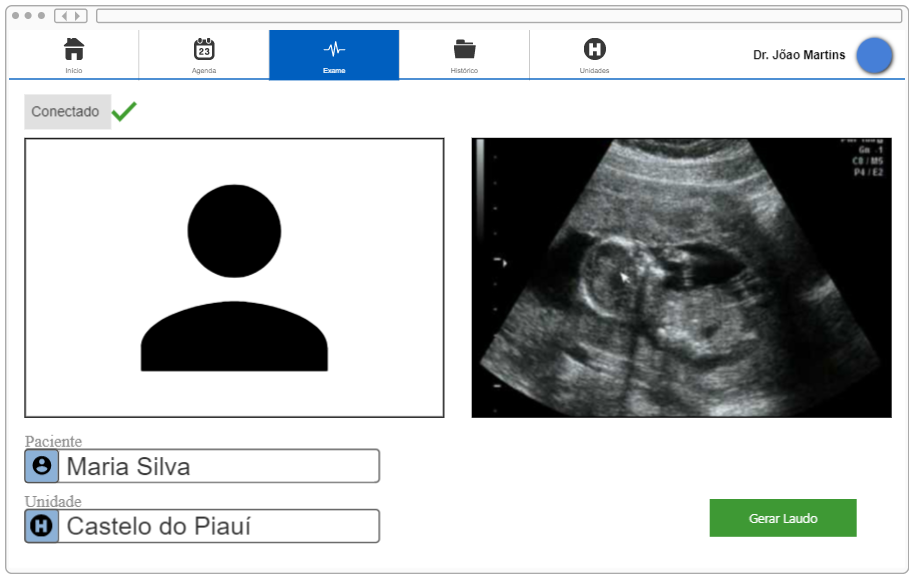
\includegraphics[keepaspectratio=true,scale=0.5]{figuras/3_0_exame_medico.png}
	\caption{Tela de exame visão do médico}
	\label{soft_7}
\end{figure}

Na tela do sistema escravo, o paciente poderá visualizar, na parte superior, a barra de navegação principal, onde o profissional responsável na unidade poderá navegar para a página principal do sistema, a agenda de exames marcados, a página para a realização do exame e o histórico de exames. Na parte central o paciente irá acompanhar o vídeo gerado pelo aparelho de ultrassom, e no lado direito as informações do médico que está realizando o exame. No canto inferior direito o profissional responsável da unidade poderá ter acesso ao laudo gerado pelo exame. A figura \ref{soft_8} mostra essa tela.

\begin{figure}[H]
	\centering	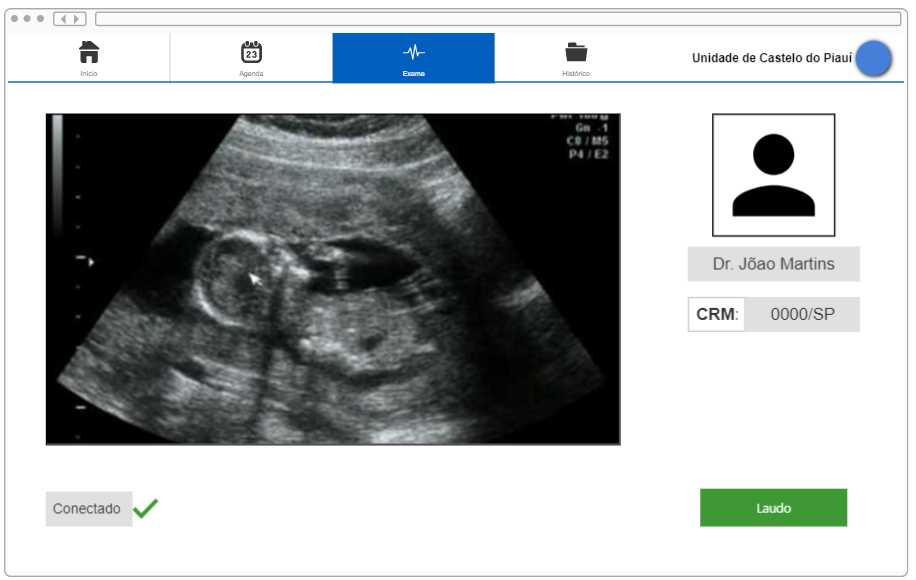
\includegraphics[keepaspectratio=true,scale=0.5]{figuras/3_1_exame_paciente.png}
	\caption{Tela de exame visão do do paciente}
	\label{soft_8}
\end{figure}
